\subsection{Effect of pruning, chaining, and inexact matches}\label{GLOBALsec:techniques}

\begin{figure}[t]
  \centering
  \subfloat[The effect of pruning on the runtime scaling with $n$ ($e{=}5\%$,
      $k{=}15$, exact~matches). Note that \SH and \CSH coincide almost exactly.]
      {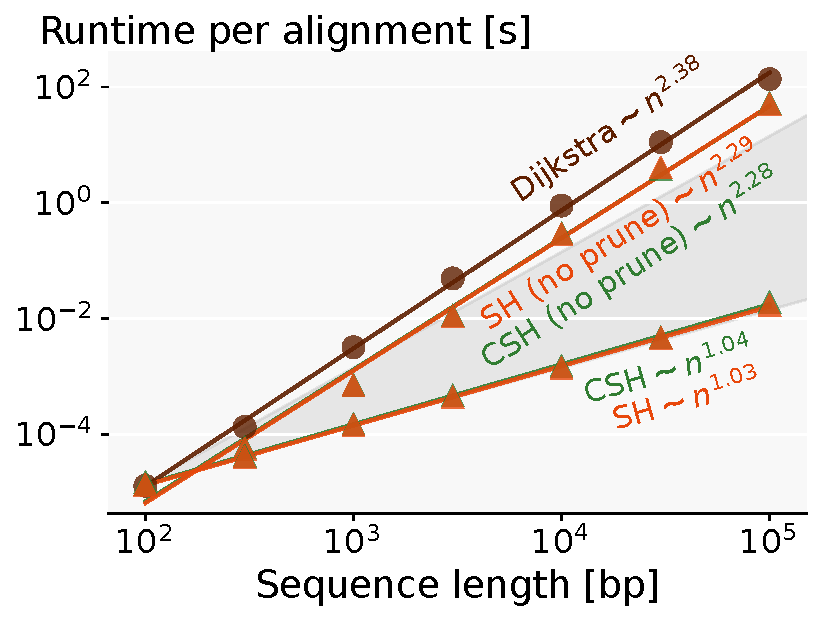
\includegraphics[width=0.45\linewidth]{imgs/fig5/scaling_n_labels.pdf}\label{GLOBALfig:scaling_n}}
  %\hfill
  \subfloat[The effect of chaining and inexact matching on the runtime scaling
  with $e$ ($n{=}10^4$, $k{=}9$, averaged over $100$ alignments).]
  {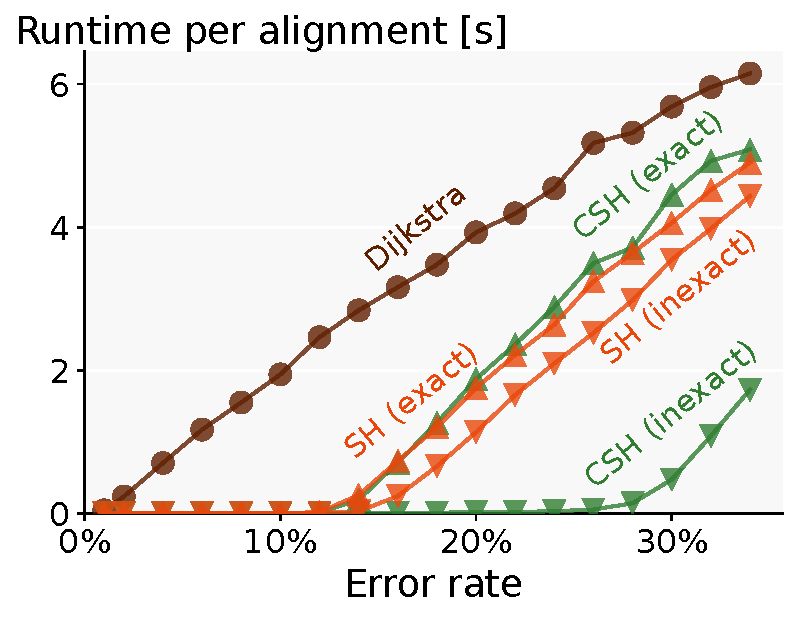
\includegraphics[width=0.45\linewidth]{imgs/fig5/scaling_e_labels.pdf}\label{GLOBALfig:scaling_e}}

  \caption[The effects of pruning, inexact matching, and chaining on runtime
   scaling with length and error rate]{The effects of seed heuristic
   optimizations on runtime scaling (\textbf{synthetic data}).}
  \label{GLOBALfig:scaling}
\end{figure}


The optimizations and generalizations of the seed heuristic~(\cref{GLOBALsec:methods})
impact the performance in a complex way. Here we aim to provide intuitive
explanations~(\cref{GLOBALfig:scaling}).

\paragraph{Pruning enables near-linear scaling with length}
\cref{GLOBALfig:scaling_n} shows that match pruning has a crucial effect on the
runtime scaling with length for both \SH and \CSH. Essentially, this
optimization changes the quadratic runtime to near-linear runtime. The pruned
variants of \SH and \CSH are averaged over $\lfloor 10^7 / n \rfloor$ sequence pairs,
while the no-prune variants and \dijkstra are averaged over $\lfloor 10^5 / n
\rfloor$ pairs.

\paragraph{Inexact matching and match chaining enable scaling to high error rates}
\cref{GLOBALfig:scaling_e} shows that inexact matches can tolerate higher error rates.
Because of the larger number of matches, chaining is needed to preserve the
near-linear runtime. There are two distinctive modes of operation: the runtime
is close to constant up to a certain error rate, after which the runtime grows
linearly in $e$. Thus, our heuristics can direct the search up to a certain
fraction of errors, after which does a \dijkstra-like exploration step for each
additional error. A reasonable quantification of the effect of different
optimizations is to mark the error rate at which the heuristic transfers to the
second (slow) mode of operation. For $n{=}10^4$ and $k{=}9$, \dijkstra starts a
linear exploration at $e{=}0\%$, \SH and \CSH with exact matches start at around
$12\%$, \SH with inexact matches start at around $14\%$, and \CSH with inexact
matches start at around $27\%$.

%The jumps in the graphs, especially visible for \dijkstra, are caused by layers
%of memory caches being exhausted.

% We choose $n{=}10^4$ since it is not near the limit for any of \sh and \csh. In
% order to highlight the difference between \sh and \csh, we choose a smaller
% value $k{=}2$, which is suboptimal for longer $n$.

%Supplementaries
%- Expanded states/band, Expanded states 1.00 scaling, h0 for SH+pruning and CSH+pruning for different e
%In the supplementaries~\cref{GLOBALsec:supplementaries} we study in detail the
%scaling of \sh and \csh with $n$ and $\spot$.
%- h0 approximate $72\%$ of $e$
%\paragraph{Internal for \sh}
